\documentclass{article}
\usepackage{amsmath}
\usepackage{amsthm}
\usepackage{enumerate}
\usepackage[bookmarks=true]{hyperref}
\usepackage{bookmark}
\usepackage{graphicx}
\usepackage{multirow}
\usepackage{color}
\usepackage[dvipsnames]{xcolor}

\newif\ifALL

\ALLtrue

\usepackage{amssymb,amsmath,amsthm,amsfonts}
\usepackage{mathrsfs}
\usepackage{dsfont}
\usepackage{enumerate}

%\newtheorem{mdef}{Definition}
%\newtheorem{theorem}{Theorem}
\newcommand{\eqsplit}[2]{
  \begin{equation}\label{#2}
    \begin{split}
      #1
    \end{split}
  \end{equation}}
\newcommand{\eqnsplit}[1]{
  \begin{eqnarray*}
    #1
  \end{eqnarray*}}
\newcommand{\tran}[1]{
  \tilde{#1}
}
\newcommand{\td}[2]{
  \frac{d #1}{d #2}
}
\newcommand{\pd}[2]{
  \frac{\partial #1}{\partial #2}
}
\newcommand{\ppd}[2]{
  \frac{\partial^2 #1}{\partial #2^2}
}
\newcommand{\pdd}[3]{
  \frac{\partial^2 #1}{\partial #2 \partial #3}
}
\newcommand{\otd}[1]{
  \frac{d}{d #1}
}
\newcommand{\opd}[1]{
  \frac{\partial}{\partial #1}
}
\newcommand{\oppd}[1]{
  \frac{\partial^2}{\partial #1^2}
}
\newcommand{\opdd}[2]{
  \frac{\partial^2}{\partial #1 \partial #2}
}
\newcommand{\ket}[1]{
  |#1\rangle
}
\newcommand{\bra}[1]{
  \langle#1|
}
\newcommand{\inn}[1]{
  \langle#1\rangle
}
\newcommand{\mean}[1]{
  \langle#1\rangle
}
\newcommand{\tr}{
  \text{tr}\,
}
\newcommand{\re}{
  \text{Re}\,
}
\newcommand\im{
  \text{Im}\,
}
\newcommand{\var}{
  \text{var}
}
\newcommand{\arcsinh}{
  \sinh^{-1}
}
\newcommand{\arccosh}{
  \cosh^{-1}
}
\newcommand{\erfc}{
  \text{erfc}
}
\newcommand{\E}{
  \mathbb{E}
}
\renewcommand{\P}{
  \mathbb{P}
}
\newcommand{\I}[1]{
  \mathbf{1}_{\{#1\}}
}
\newcommand{\1}[1]{
  \mathds{1}_{\{#1\}}
}
\newcommand{\diag}{
  \text{diag\,}
}
\newcommand{\M}{
  {\text{max}}
}
\newcommand{\m}{
  {\text{min}}
}
\newcommand{\ph}{
  {\text{arg}\,}
}
\newcommand\erf{
  \text{erf}
}
\renewcommand\vec[1]{
  \mathbf{#1}
}
\newcommand\mtx[1]{
  \mathbf{#1}
}
\newcommand\ed{
  \,{\buildrel d \over =}\,
}



\title{To be Determined}
\author{Xie Xiaolei}
\date{\today}
\begin{document}
\maketitle

\section{Introduction}
We study the covariance matrix of a $p$-dimensional sequence with each
component modeled by a GARCH(1, 1) process:

\begin{eqnarray*}
  X_{i,t} &=& \sigma_{i,t} Z_{i,t} \\
  (Z_{1, t}, Z_{2,t}, \dots, Z_{p,t}) &\sim& N(0, \Sigma) \\
  \sigma_{i, t}^2 &=& \omega_i + \alpha_i X_{i, t-1}^2 + \beta_i
  \sigma_{i, t-1}^2
\end{eqnarray*}

\section{IGARCH(1) Processes}
We first consider the cases where $\alpha_i + \beta_i = 1$,
i.e. IGARCH models.

\subsection{IARCH(1)}
In this case $\alpha_i = 1$, $\beta_i = 0$. Thus, from the equation
\begin{equation*}
  \E (Z_i^2)^{\xi_i} = 1
\end{equation*}
we obtain $\xi_i = 1$. Suppose
\begin{eqnarray*}
  \E (Z_i^2 Z_j^2)^{\xi/2} &=& 1 \\
  (Z_i, Z_j) &\sim& N(0, \Sigma) \\
  \Sigma &=&
  \begin{pmatrix}
    1 & \rho \\
    \rho & 1
  \end{pmatrix}
\end{eqnarray*}
Re-writing the above equation gives
\begin{equation}
  \label{eq:iarch1_1st}
  {1 \over 2\pi}
  \int \int
  \left(
    \rho^2 x^4 + (1 - \rho^2) x^2 y^2 + 2 \rho \sqrt{1 - \rho^2} x^3 y
  \right)^{\xi/2}
  \exp\left(
    -{x^2 + y^2 \over 2}
  \right)
  dx dy = 1
\end{equation}
When $\rho = \pm 1$, it is clear $\xi = 1$. When $-1 < \rho < 1$,
we may re-write \eqref{eq:iarch1_1st} in polar coordinates to obtain
\begin{equation*}
  {1 \over 2\pi} \int_0^{\infty} r^{2\xi + 1} e^{-r^2 / 2} dr
  \int_{0}^{2\pi} \cos(\theta)^{\xi}
  \left(
    2 \rho^2 \cos(\theta)^2
    + 2 \rho \sqrt{1 - \rho^2} \cos(\theta) \sin(\theta) -
    \cos(\theta)^2 + 1 - \rho^2
  \right)^{\xi/2} d\theta = 1
\end{equation*}
Integrating the radial part of the integral results in
\begin{equation*}
  \int_{0}^{2\pi}
  \cos(\theta)^{\xi}
  \left(
    2 \rho^2 \cos(\theta)^2 + \rho \sqrt{1 - \rho^2} \sin(2\theta) -
    \cos(\theta)^2 - \rho^2 + 1
  \right)^{\xi/2} d\theta
  = {2 \pi
    \over
    2^{\xi} \Gamma(\xi + 1)
  }
\end{equation*}
After some manipulations we arrive at
\begin{equation}
  \label{eq:iarch_2nd}
  \int_{-1}^1 (\sin(\pi z) + \rho)^{\xi} dz = {2 \over \Gamma(\xi + 1)}
\end{equation}
Using this result, we immediately obtain for ARCH(1) models
\begin{equation}
  \label{eq:arch_1st}
  \int_{-1}^1 (\sin(\pi z) + \rho)^{\xi} dz =
  {2 \over \Gamma(\xi + 1)}
  {1 \over (\alpha_i \alpha_j)^{\xi/2}}
\end{equation}
Fitting ARCH(1) models to the FX return series and then simulating the
models produces a fairly good match between the spectra of the
simulated and the real series, as shown in figure
\ref{fig:FX_ARCH_eigenvalues} and \ref{fig:FX_ARCH_eigenvectors}.
\begin{figure}[htb!]
  \centering
  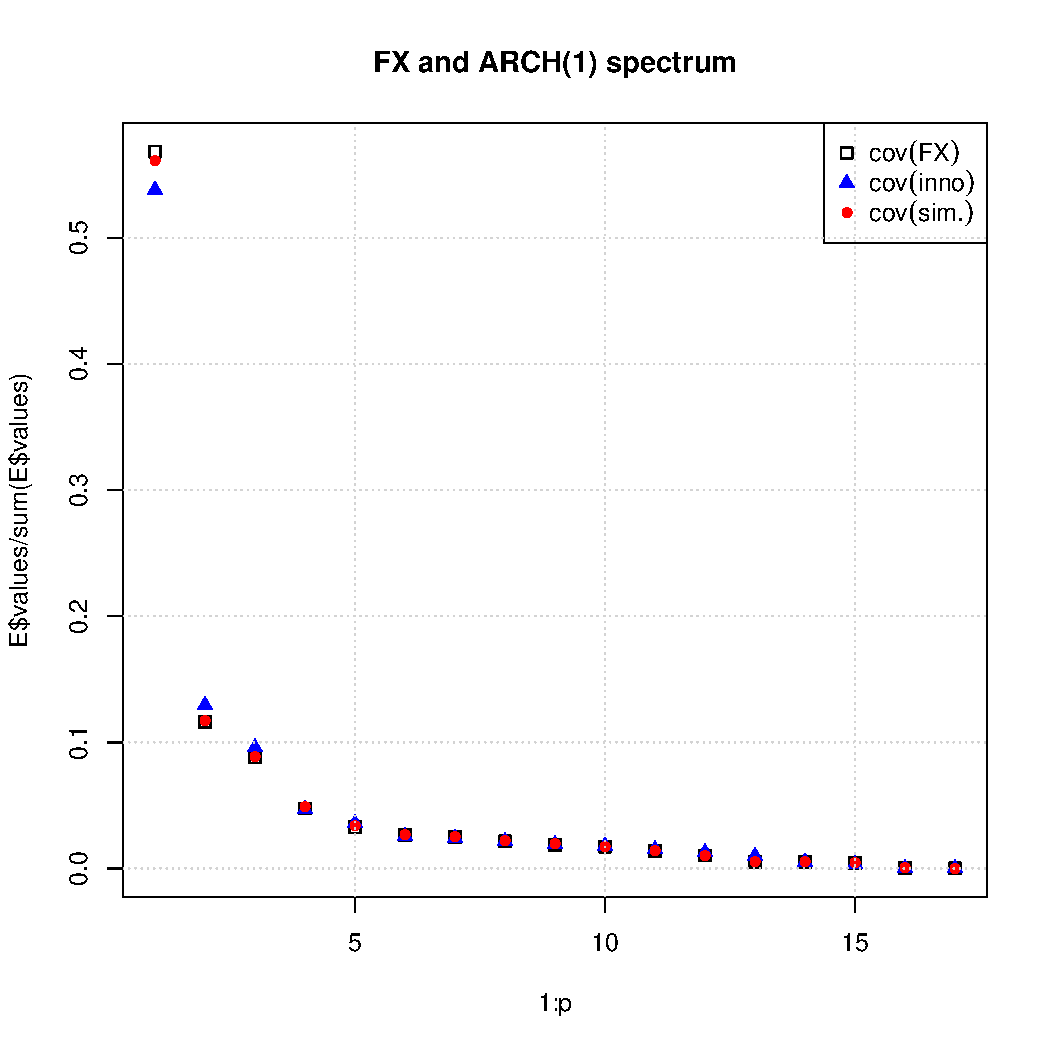
\includegraphics[scale=0.4]{FX_eigenvalues.pdf}  
  \caption{FX \& simulated ARCH eigenvalues}
  \label{fig:FX_ARCH_eigenvalues}
\end{figure}

\begin{figure}[htb!]
  \centering
  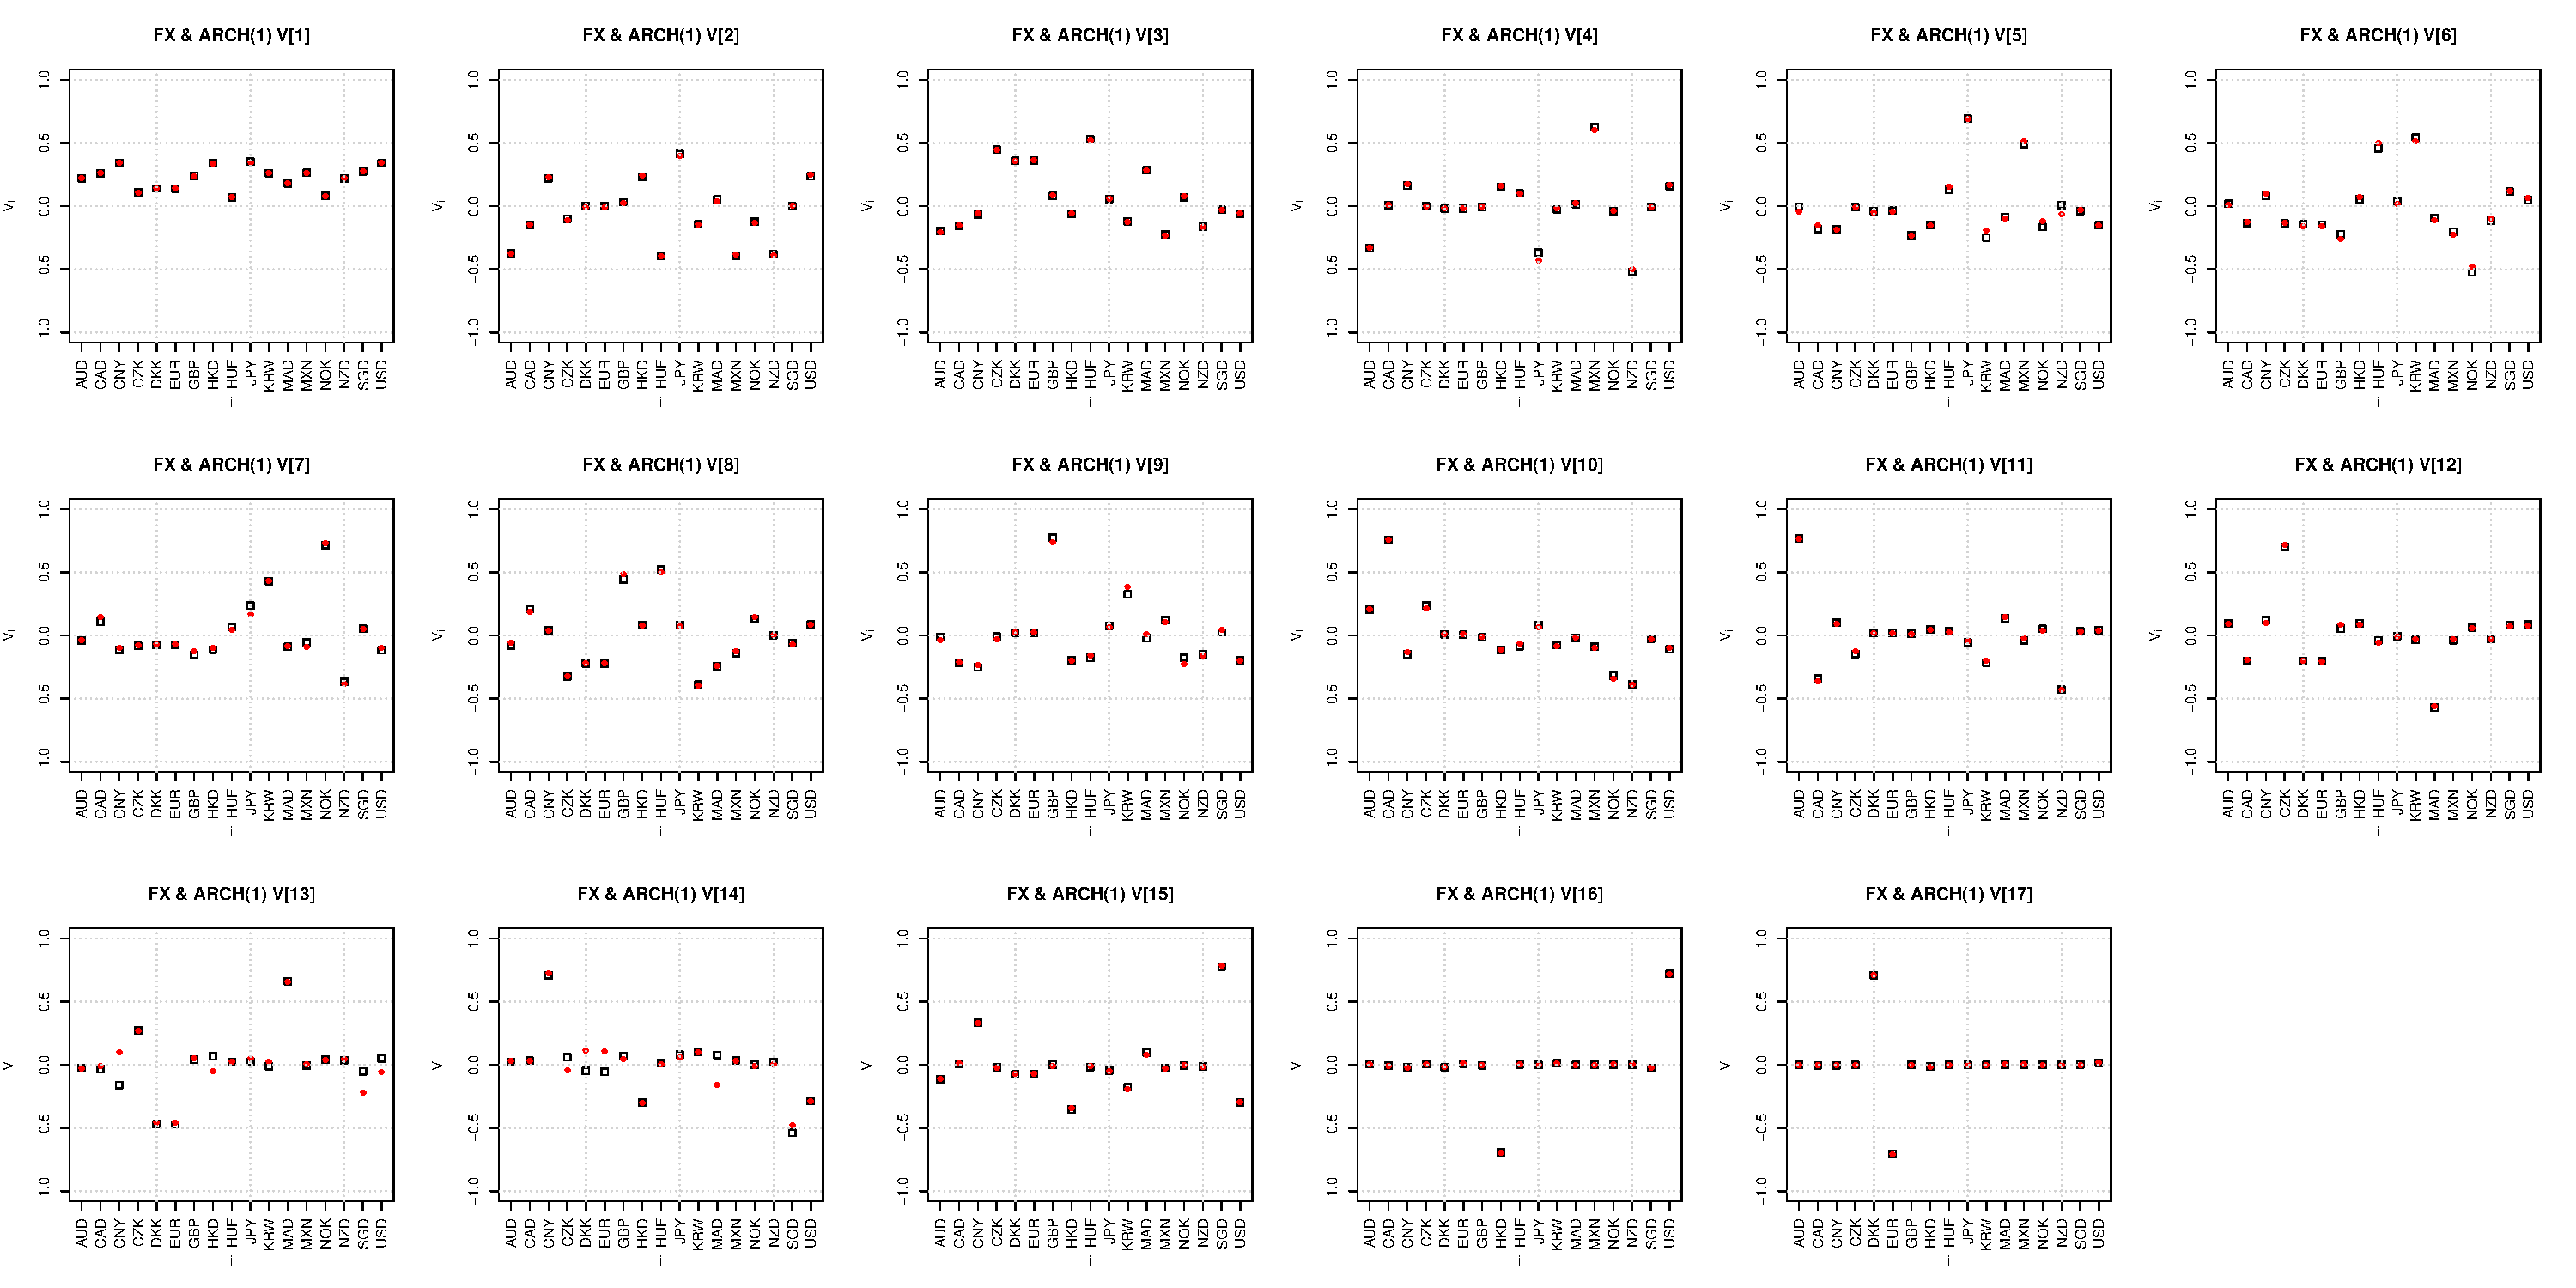
\includegraphics[scale=0.3]{FX_eigenvectors.pdf}  
  \caption{FX \& ARCH eigenvectors}
  \label{fig:FX_ARCH_eigenvectors}
\end{figure}

To compare the solution to \eqref{eq:arch_1st}, call it $\xi_{i,j}$
with the tail indices of $\text{ARCH}(1)$ processes with parameters
$\alpha_i$ and $\alpha_j$, we fix $\alpha_i \alpha_j$ and let
$\alpha_i = \alpha_j = \sqrt{\alpha_i \alpha_j}$. Since $\xi_i$ as a
function of $\alpha_i$ is monotonically decreasing, $\min\{\xi_i,
\xi_j\}$ is at its maximum when $\alpha_i = \alpha_j$ for fixed
$\alpha_i \alpha_j$. This is the reason for the above setup. Table
\ref{tab:tail_indices_normal} lists the values of $\xi_i$ and
$\xi_{i,j}$. Here $\text{corr}(Z_i, Z_j)$ varies from 0.09 to 0.99.
\begin{table}[htb!]
  \centering
  \begin{scriptsize}
  \begin{tabular}{c|c|cccccccccc}
    \multicolumn{2}{c|}{$\alpha_i \alpha_j$} & 0.090 & 0.190 & 0.290 &
    0.390 & 0.490 & 0.590 & 0.690 & 0.790 & 0.890 & 0.990 \\
    \hline
    \multicolumn{2}{c|}{$\alpha_i, \alpha_j$} & 0.300 & 0.436 & 0.539 &
    0.624 & 0.700 & 0.768 & 0.831 & 0.889 & 0.943 & 0.995 \\
    \hline
    \multicolumn{2}{c|}{$\xi_i, \xi_j$} & 4.180 & 2.766 & 2.170 &
    1.822 & 1.586 & 1.413 & 1.279 & 1.171 & 1.082 & 1.007 \\
    \hline
    \multirow{10}{*}{$\text{corr}(Z_i Z_j)$} & 0.1 & 8.041 & 5.375 &
    4.238 & 3.568 &
    3.113 & 2.778 & 2.518 & 2.308 & 2.134 & 1.987 \\
    & 0.2 & 7.439 & 5.031 & 3.997 & 3.384 & 2.964 &
    2.653 & 2.411 & 2.215 & 2.052 & 1.914 \\
    & 0.3 & 6.846 & 4.652 & 3.713 & 3.156 &
    2.774 & 2.491 & 2.269 & 2.089 & 1.939 & 1.812 \\
    & 0.4 & 6.318 & 4.294 & 3.434 & 2.924 &
    2.575 & 2.317 & 2.114 & 1.950 & 1.813 & 1.696 \\
    & 0.5 & 5.852 & 3.970 & 3.174 & 2.704 &
    2.383 & 2.146 & 1.960 & 1.810 & 1.684 & 1.577 \\
    & 0.6 & 5.441 & 3.679 & 2.936 & 2.500 &
    2.203 & 1.983 & 1.812 & 1.673 & 1.558 & 1.460 \\
    & 0.7 & 5.074 & 3.417 & 2.720 & 2.312 &
    2.035 & 1.830 & 1.671 & 1.543 & 1.436 & 1.345 \\
    & 0.8 & 4.746 & 3.180 & 2.522 & 2.138 &
    1.877 & 1.686 & 1.537 & 1.418 & 1.318 & 1.234 \\
    & 0.9 & 4.449 & 2.964 & 2.340 & 1.975 &
    1.729 & 1.548 & 1.408 & 1.296 & 1.203 & 1.124 \\
    & 1.0 & 4.180 & 2.766 & 2.170 & 1.822 &
    1.586 & 1.413 & 1.279 & 1.171 & 1.082 & 1.007
  \end{tabular}
  \end{scriptsize}
  \caption{$\xi_i, \xi_j$ and $\xi_{i,j}$}
  \label{tab:tail_indices_normal}
\end{table}


\section{General IGARCH(1)}
For general IGARCH(1) models, the equation
\begin{equation*}
  \E \left[
    (
    \alpha_i Z_1^2 + 1 - \alpha_i
    )^{\xi/2}
    (
    \alpha_j Z_2^2 + 1 - \alpha_j
    )^\xi\right] = 1
\end{equation*}
has to be solved numerically. Figure \ref{fig:xi_rho0.5} shows $\xi$
as a function of $(\alpha_i, \alpha_j)$ as defined by the
above equation.
\begin{figure}[htb!]
  \centering
  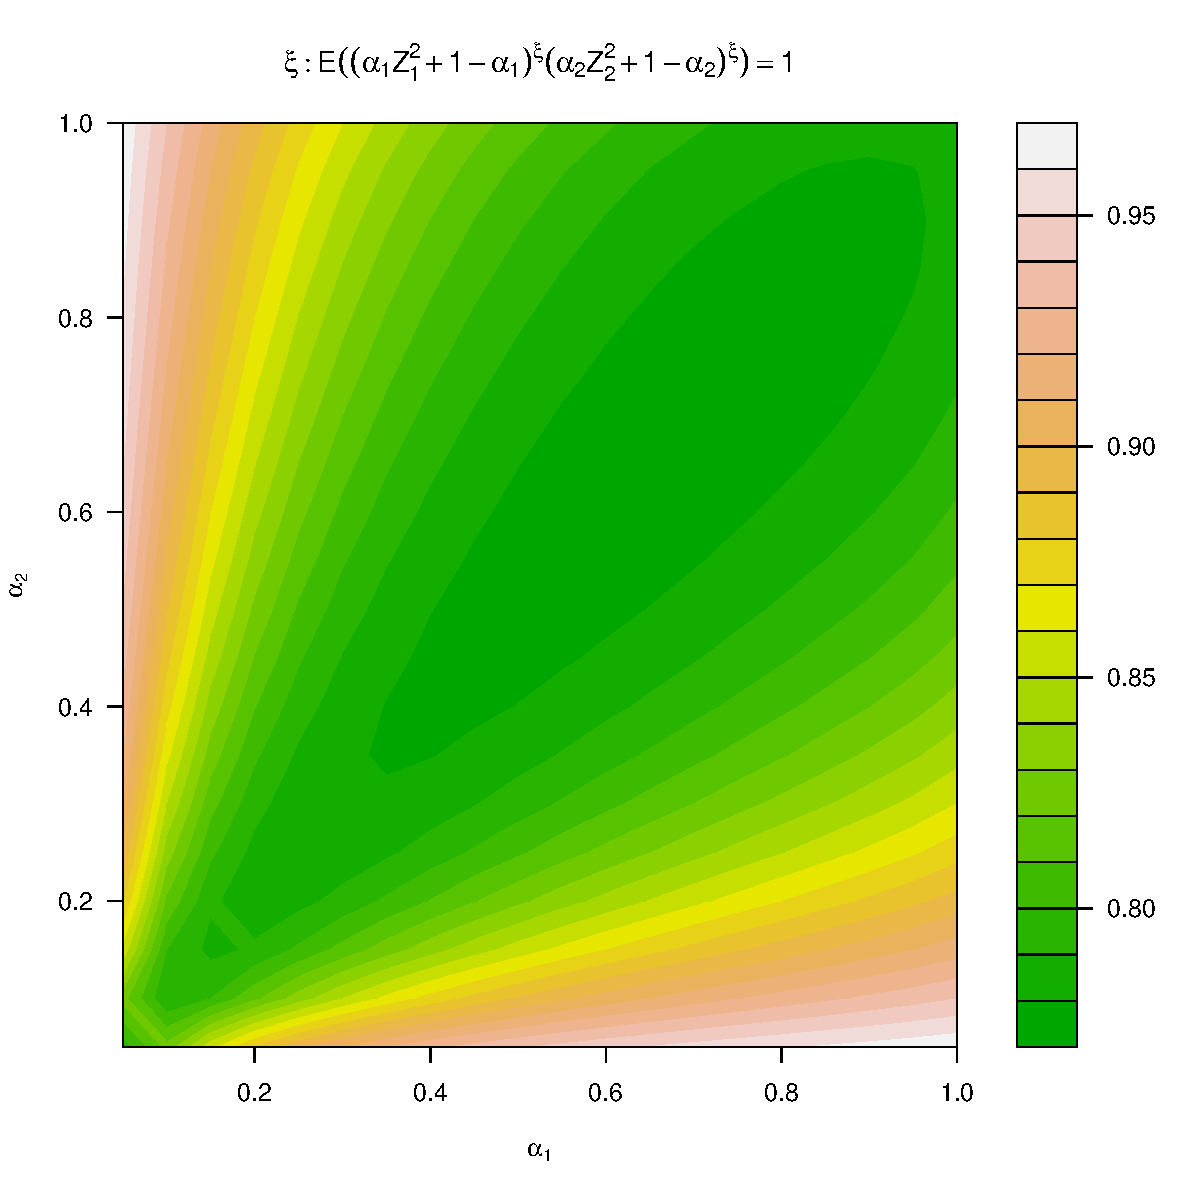
\includegraphics[scale=0.4]{igarch_rho0dot5.pdf}
  \caption{$\xi(\alpha_1, \alpha_2)$ for $\rho = 1/2$}
  \label{fig:xi_rho0.5}
\end{figure}

\section{Heavy-Tailed Innovations}
Figure \ref{fig:ARCH_t_FX_eigenvalues} and Figure
\ref{fig:ARCH_t_FX_eigenvectors} show the eigenvalues and
eigenvectors of the simulated GARCH(1, 1) process with innovations
following t(4) distribution. Clearly, the spectrum of the simulated
series does not match that of the observed FX series.
\begin{figure}[htb!]
  \centering
  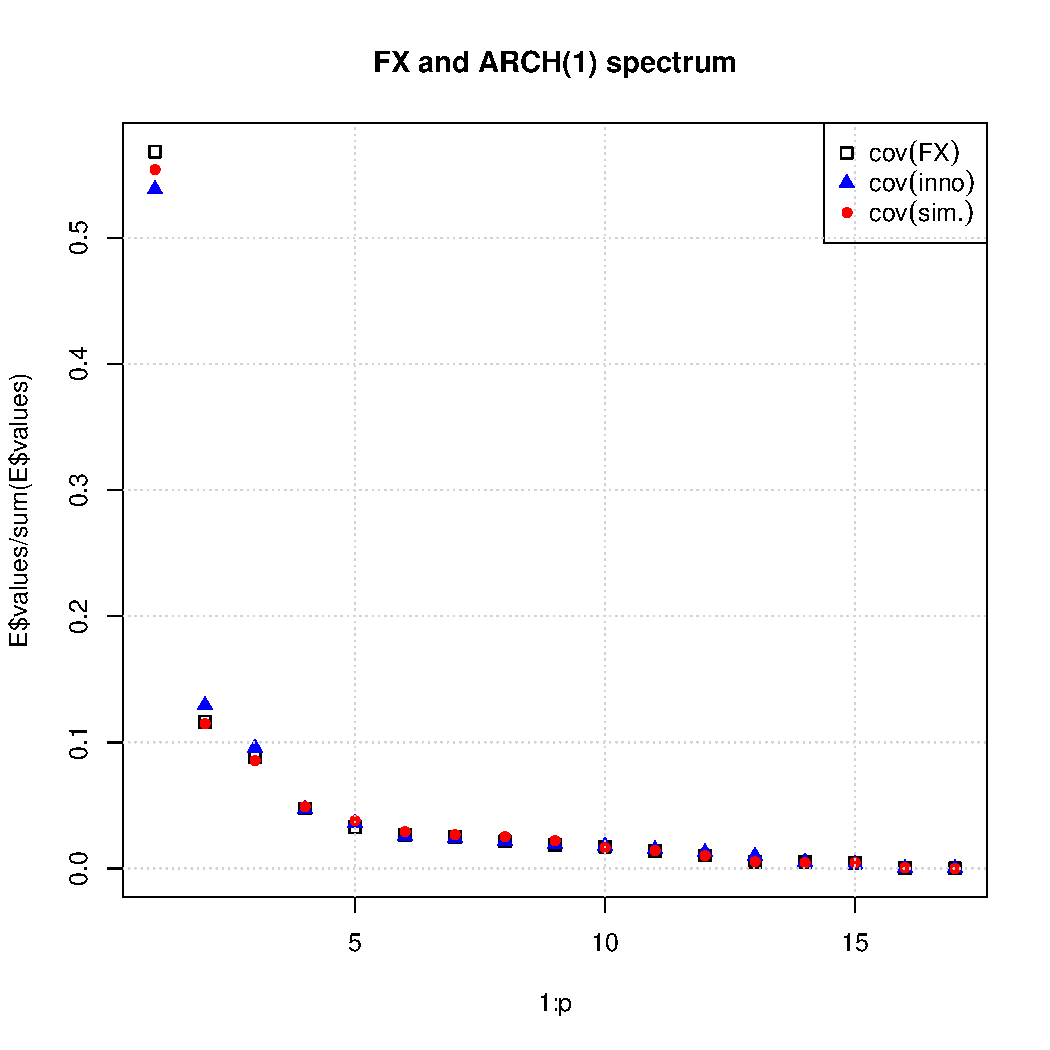
\includegraphics[scale=0.4]{FX_eigenvalues_ARCH_t_inno.pdf}  
  \caption{FX \& simulated ARCH eigenvalues. t-distributed innovations}
  \label{fig:ARCH_t_FX_eigenvalues}
\end{figure}

\begin{figure}[htb!]
  \centering
  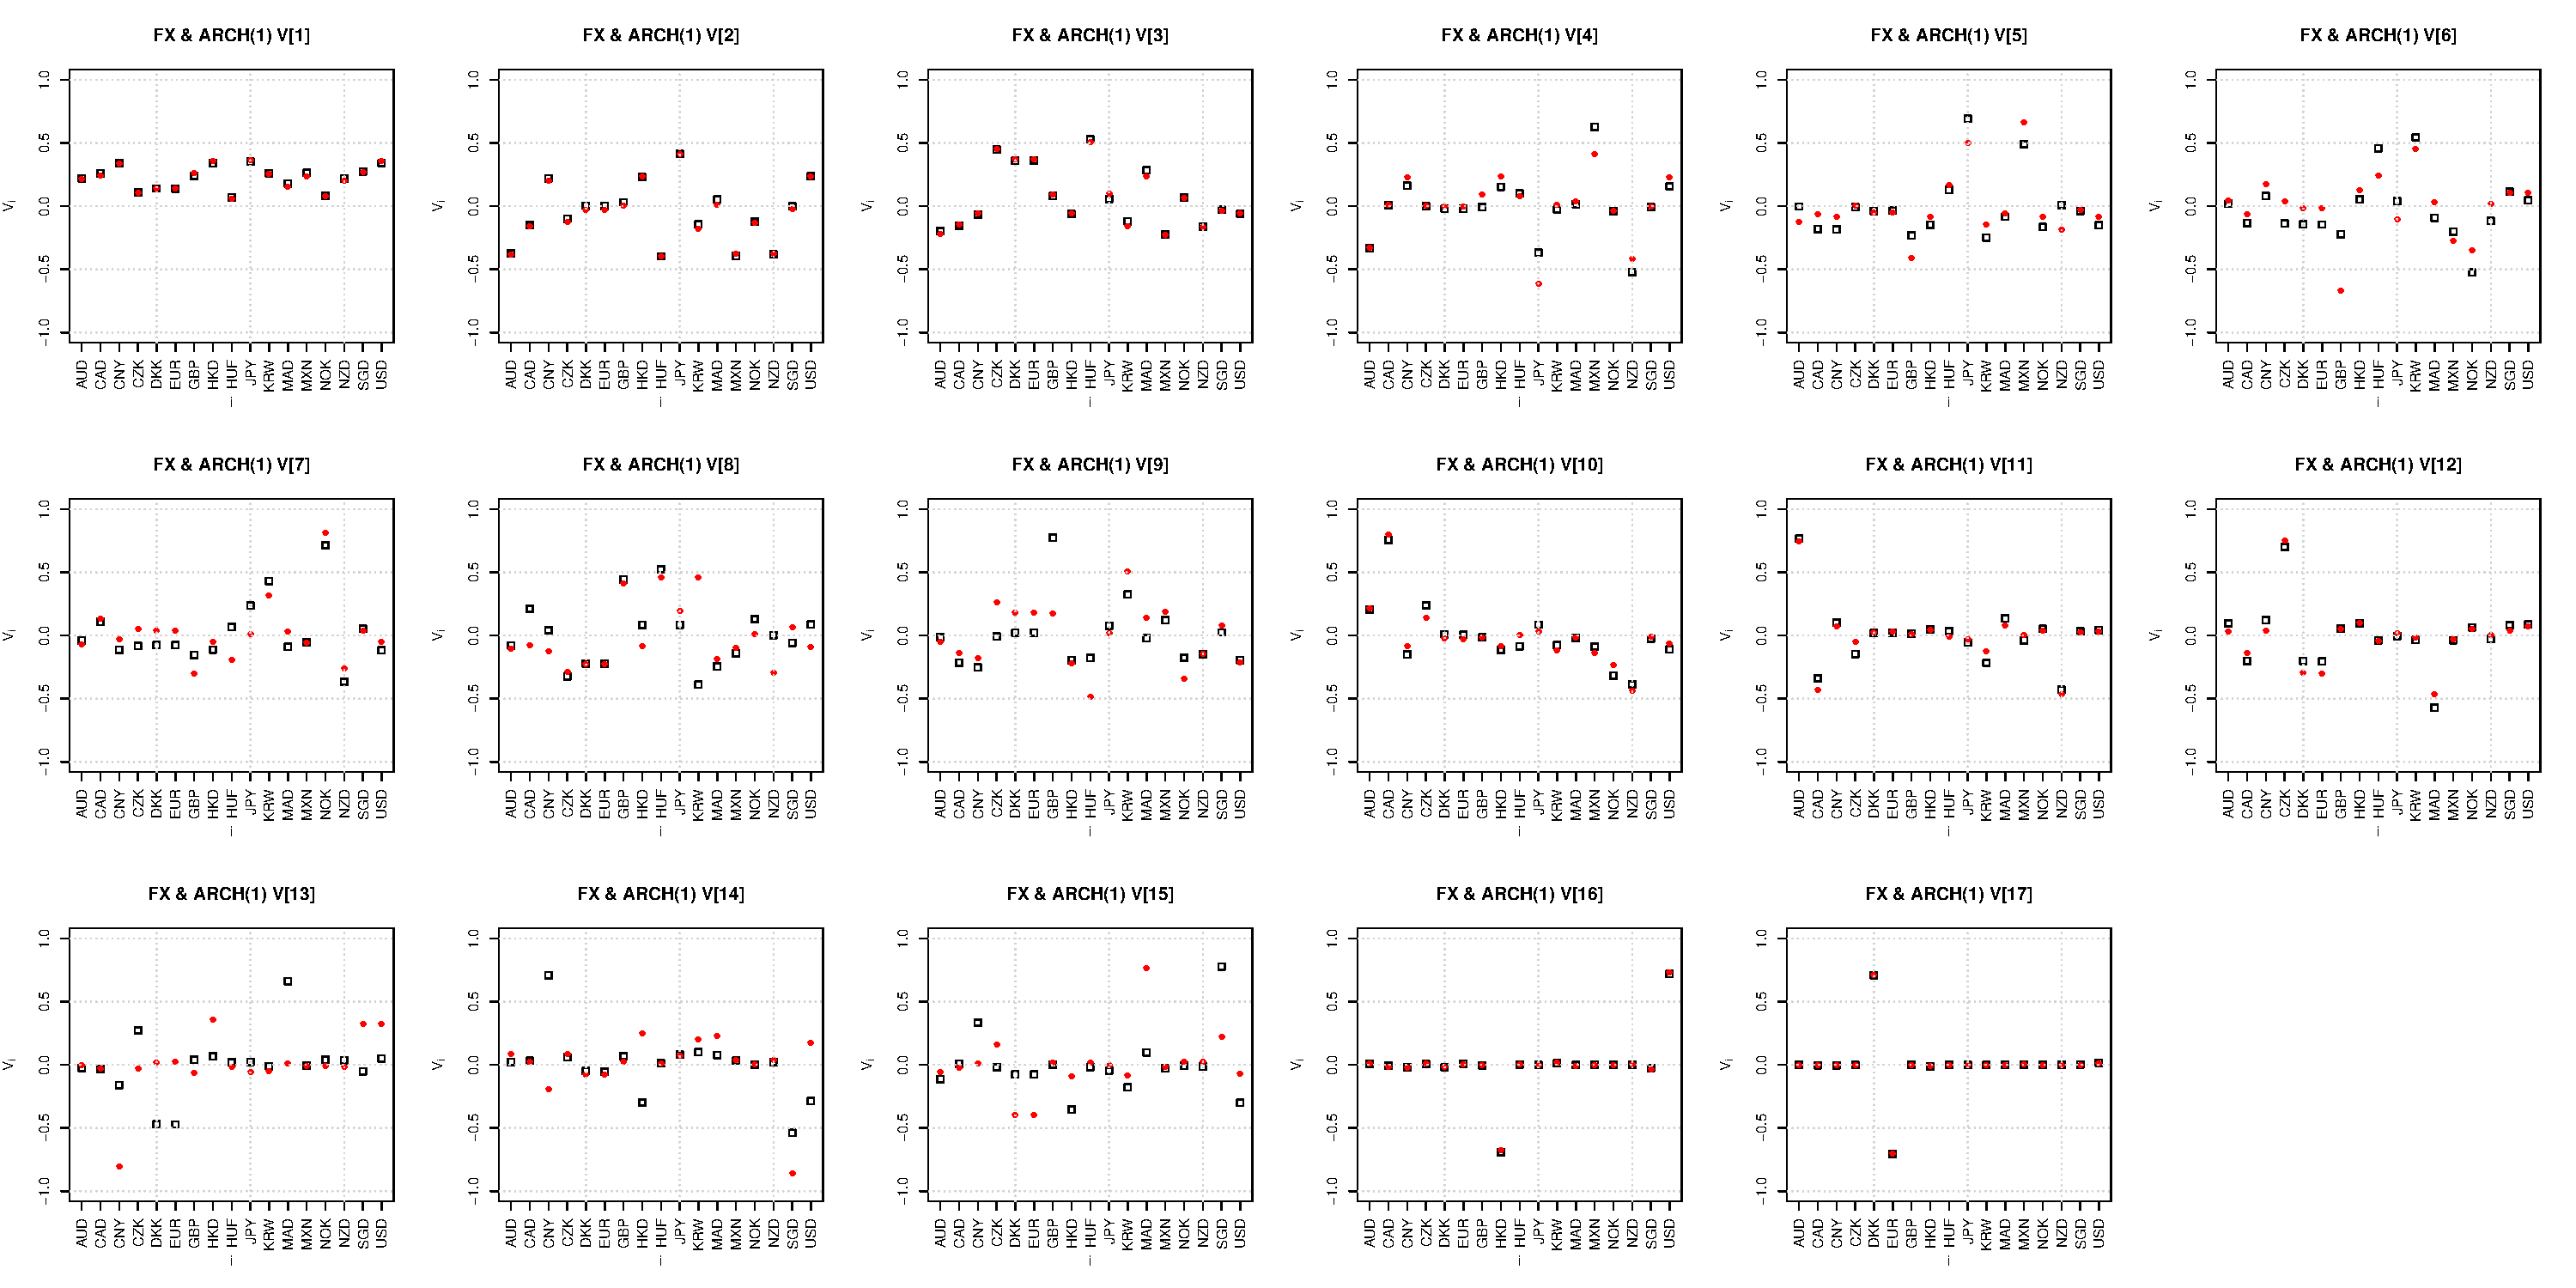
\includegraphics[scale=0.3]{FX_eigenvectors_ARCH_t_inno.pdf}  
  \caption{FX \& ARCH eigenvectors. t-distributed innovations}
  \label{fig:ARCH_t_FX_eigenvectors}
\end{figure}

On the other hand, if each series $X_{i,t}$ is assumed to have
conditional distribution $t(\nu_i)$ with $\nu_i, \nu_j$ potentially
different from each other, the following parameters as listed in table
\ref{tab:ARCH_t_params} are obtained:
\begin{table}[htb!]
  \centering
  \begin{tabular}{c|cccc}
    currency & $\omega$ & $\alpha$ & $\beta$ & $\nu$ \\
    \hline
    AUD & 1.1e-06 & 0.026 & 0.949 & 9.8 \\
    CAD & 2.1e-07 & 0.015 & 0.980 & 8.3 \\
    CNY & 2.6e-07 & 0.038 & 0.957 & 7.0 \\
    CZK & 2.4e-07 & 0.035 & 0.955 & 8.3 \\
    DKK & 6.5e-07 & 0.060 & 0.905 & 9.5 \\
    EUR & 6.3e-07 & 0.061 & 0.905 & 9.6 \\
    GBP & 7.9e-07 & 0.049 & 0.931 & 10.0 \\
    HKD & 2.6e-07 & 0.041 & 0.955 & 8.8 \\
    HUF & 5.8e-07 & 0.045 & 0.942 & 7.5 \\
    JPY & 5.4e-07 & 0.052 & 0.942 & 8.5 \\
    KRW & 1.4e-06 & 0.053 & 0.916 & 6.8 \\
    MAD & 5.8e-07 & 0.045 & 0.938 & 3.7 \\
    MXN & 3.8e-06 & 0.083 & 0.875 & 3.9 \\
    NOK & 1.6e-07 & 0.030 & 0.962 & 6.7 \\
    NZD & 4.3e-07 & 0.020 & 0.972 & 10.0 \\
    SGD & 4.2e-07 & 0.040 & 0.947 & 10.0 \\
    USD & 2.5e-07 & 0.040 & 0.956 & 8.5
  \end{tabular}
  \label{tab:ARCH_t_params}
  \caption{parameters for univariate GARCH(1,1)-t models}
\end{table}

\section{Spectra of Squared returns}
Figure \ref{fig:FX_squares_eigenvalues} and
\ref{fig:FX_squares_eigenvectors} show the eigenvalues and
eigenvectors of the sample covariance matrix of squared return series
of the selected foreign exchange rates. Table
\ref{tab:FX_squared_Hill} shows the Hill estimators of $X_{i,t}^2$ and
$X_{i,t} X_{i-1,t}$.

\begin{figure}[htb!]
  \centering
  \includegraphics[scale=0.4]{FX_squares_eigenvalues.pdf}  
  \caption{Eigenvalues of sample covariance matrix of returns and
    squared returns of FX}
  \label{fig:FX_squares_eigenvalues}
\end{figure}

\begin{table}[htb!]
  \centering
  \begin{tabular}{c|c|c}
    currency & Hill est. & Hill est. of prod.\\
    \hline
    AUD & 2.129957 \\
    CAD & 2.388715 & 2.417197 \\
    CNY & 2.483576 & 2.990937 \\
    CZK & 2.341256 & 2.677970 \\
    DKK & 2.303255 & 2.873808 \\
    EUR & 2.496141 & 2.528287 \\
    GBP & 2.355945 & \textcolor{BrickRed}{1.979052} \\
    HKD & 1.814324 & 2.222141 \\
    HUF & 1.829534 & 2.308966 \\
    JPY & 1.923963 & 2.109159 \\
    KRW & 1.983916 & 2.296491 \\
    MAD & 5.000601 & 2.438606 \\
    MXN & 5.288364 & \textcolor{BrickRed}{2.063652} \\
    NOK & 1.814017 & 2.381056 \\
    NZD & 2.224353 & 2.270946 \\
    SGD & 2.003079 & 2.009848 \\
    USD & 2.268252 & 2.452259 \\
  \end{tabular}
  \caption{Hill Estimator of $X_{i,t}^2$ and $X_{i,t} X_{j,t}$}
  \label{tab:FX_squared_Hill}
\end{table}

\begin{figure}[htb!]
  \centering
  \includegraphics[scale=0.3]{FX_squares_eigenvectors.pdf}  
  \caption{Eigenvectors of sample covariance matrix of returns and
    squared returns of FX}
  \label{fig:FX_squares_eigenvectors}
\end{figure}


\section{Spectra of S\&P sectors}
\subsection{Utilities}
Fitting the daily returns' data of 25 companies that have been
included in the S\&P 500 index since 2010-01-01 and categorized in the
sector ``Utilities'', we obtained 23 GARCH(1, 1) models that satisfy
the condition
\begin{equation}
  \label{eq:garch_cond1}
  \alpha_1 + \beta_1 < 1  
\end{equation}
Then we simulate the GARCH(1, 1) processes with innovations having the
same covariance structure as those of the real data. Figure
\ref{fig:Utilities_eigenvalues} and \ref{fig:Utilities_eigenvectors1},
\ref{fig:Utilities_eigenvectors2}
compare the eigenvalues and eigenvectors, respectively, of the 
covariance matrices of the real and the simulated data.
\begin{figure}[htb!]
  \centering
  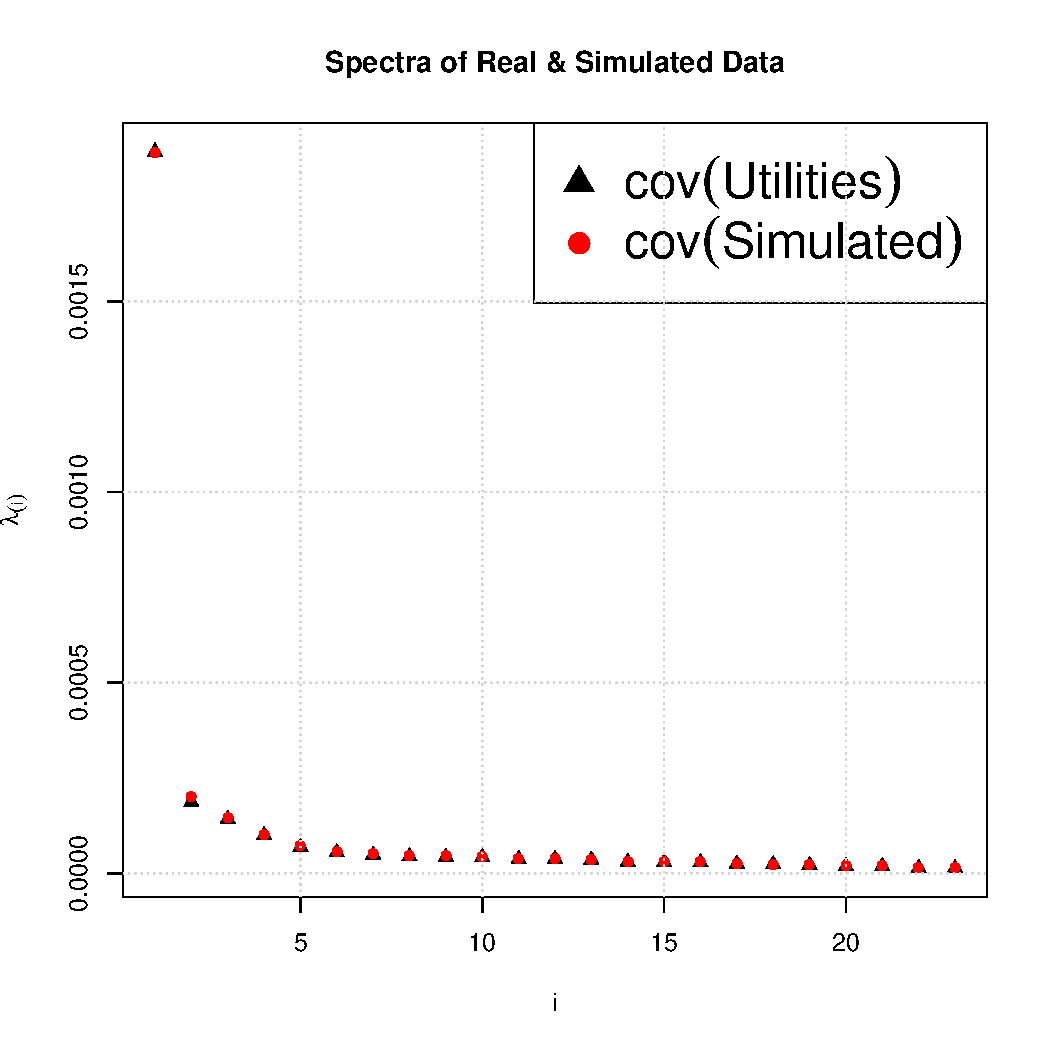
\includegraphics[scale=0.4]{Utilities_eigenvalues.pdf}
  \caption{Eigenvalues of Utilities: real \& simulated}
  \label{fig:Utilities_eigenvalues}
\end{figure}

\begin{figure}[htb!]
  \centering
  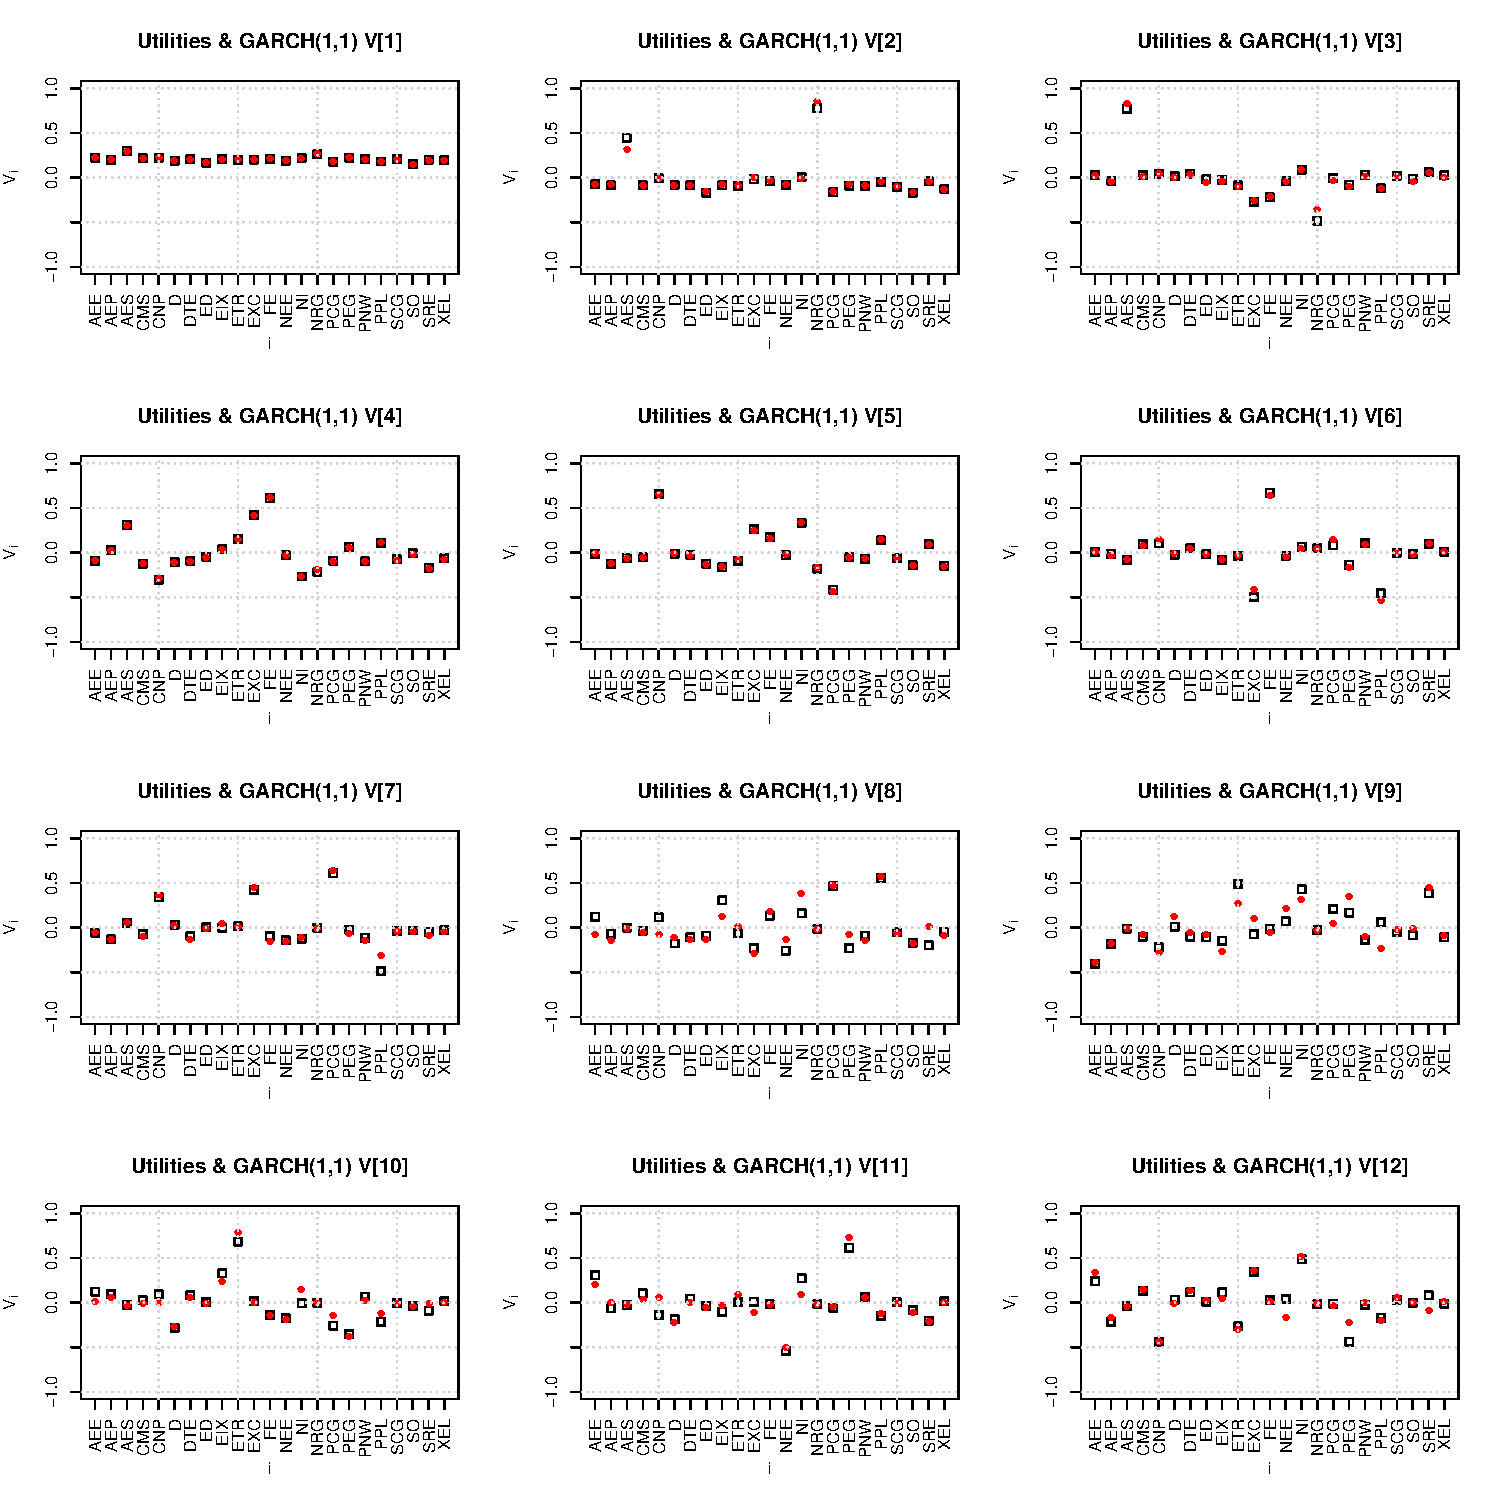
\includegraphics[scale=0.5]{Utilities_eigenvectors1.pdf}
  \caption{Eigenvectors of Utilities: real \& simulated}
  \label{fig:Utilities_eigenvectors1}
\end{figure}

\begin{figure}[htb!]
  \centering
  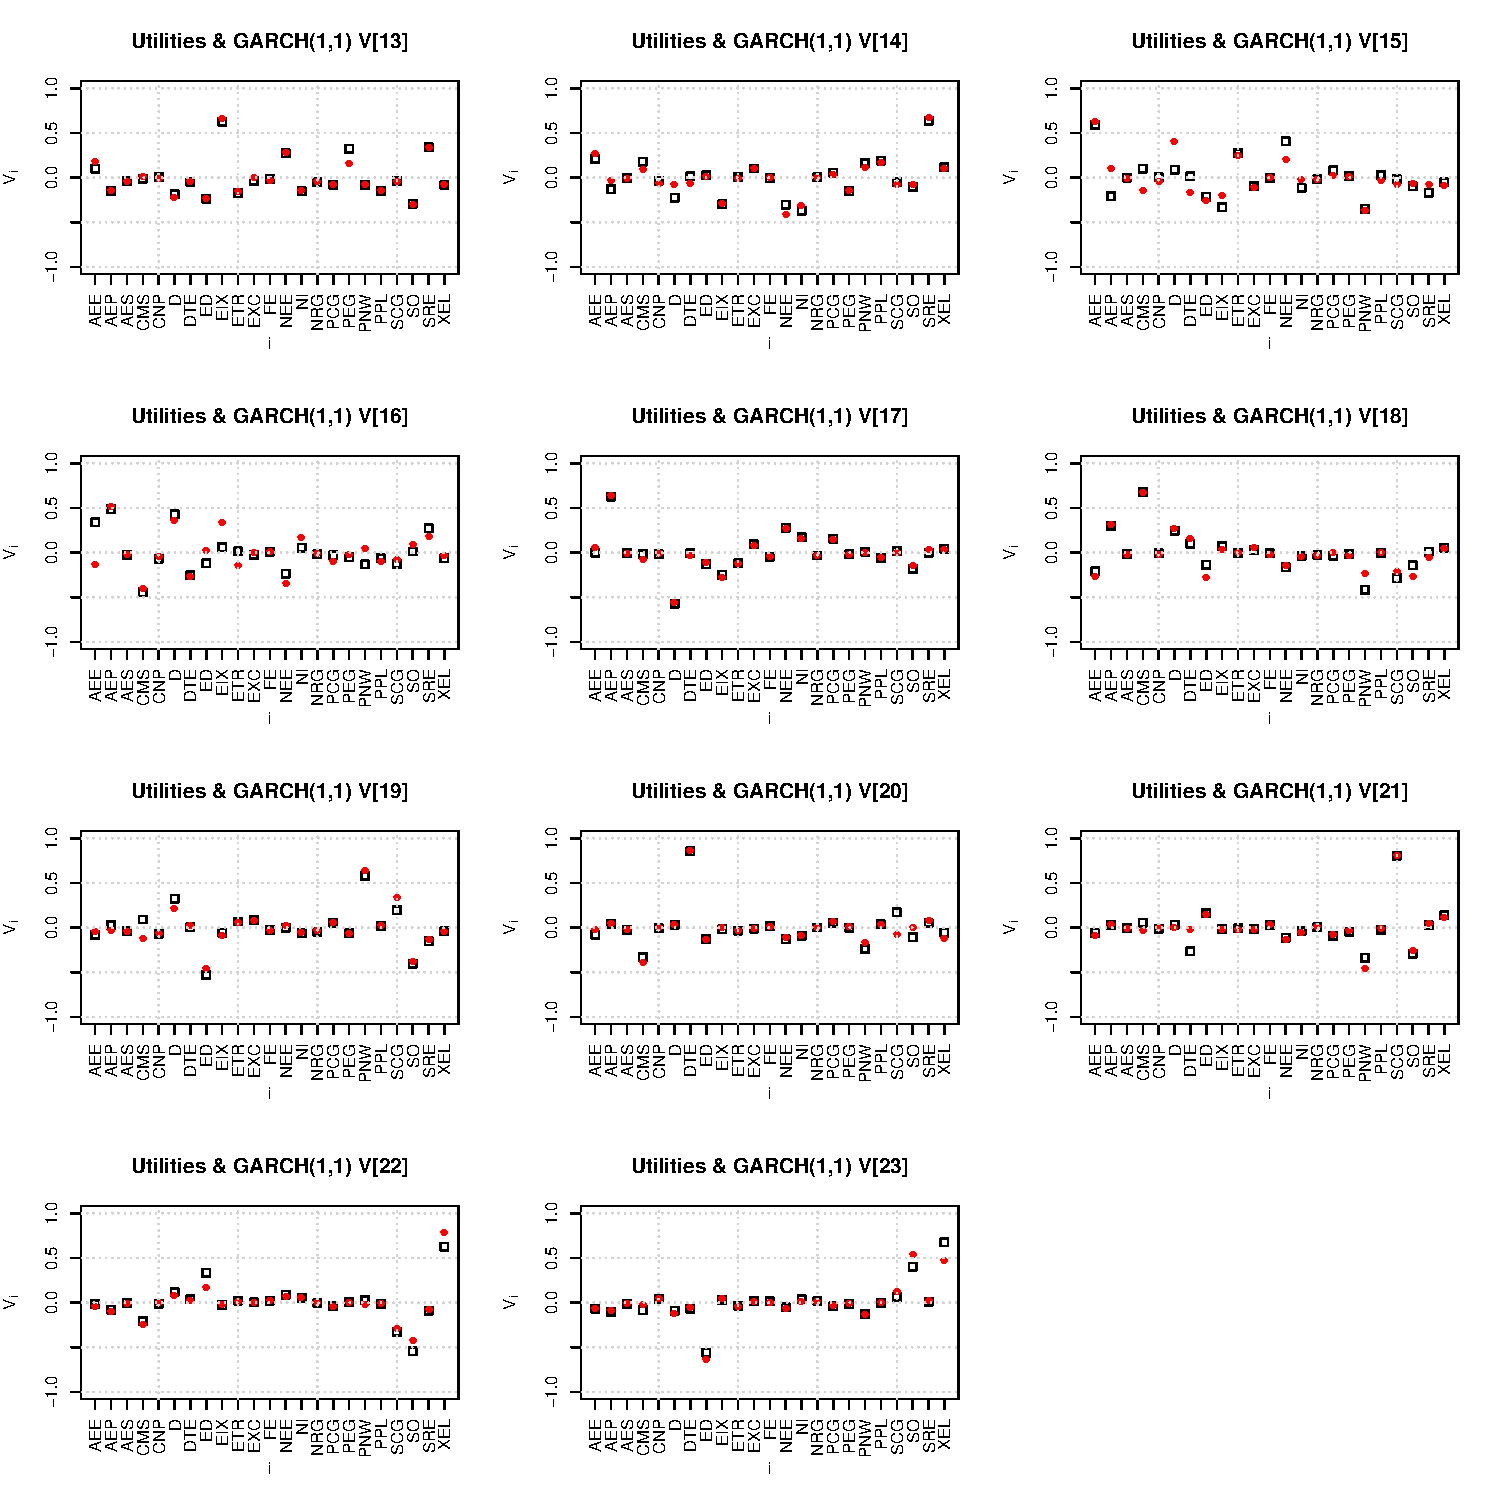
\includegraphics[scale=0.5]{Utilities_eigenvectors2.pdf}
  \caption{Eigenvectors of Utilities: real \& simulated continued}
  \label{fig:Utilities_eigenvectors2}
\end{figure}

\subsection{Materials}
A similar analysis on the ``Materials'' sector produces the following
spectra. In this sector, 21 out of 25 return sequencies are
successfully fitted to GARCH(1, 1) models that satisfy condition
\eqref{eq:garch_cond1}.

\begin{figure}[htb!]
  \centering
  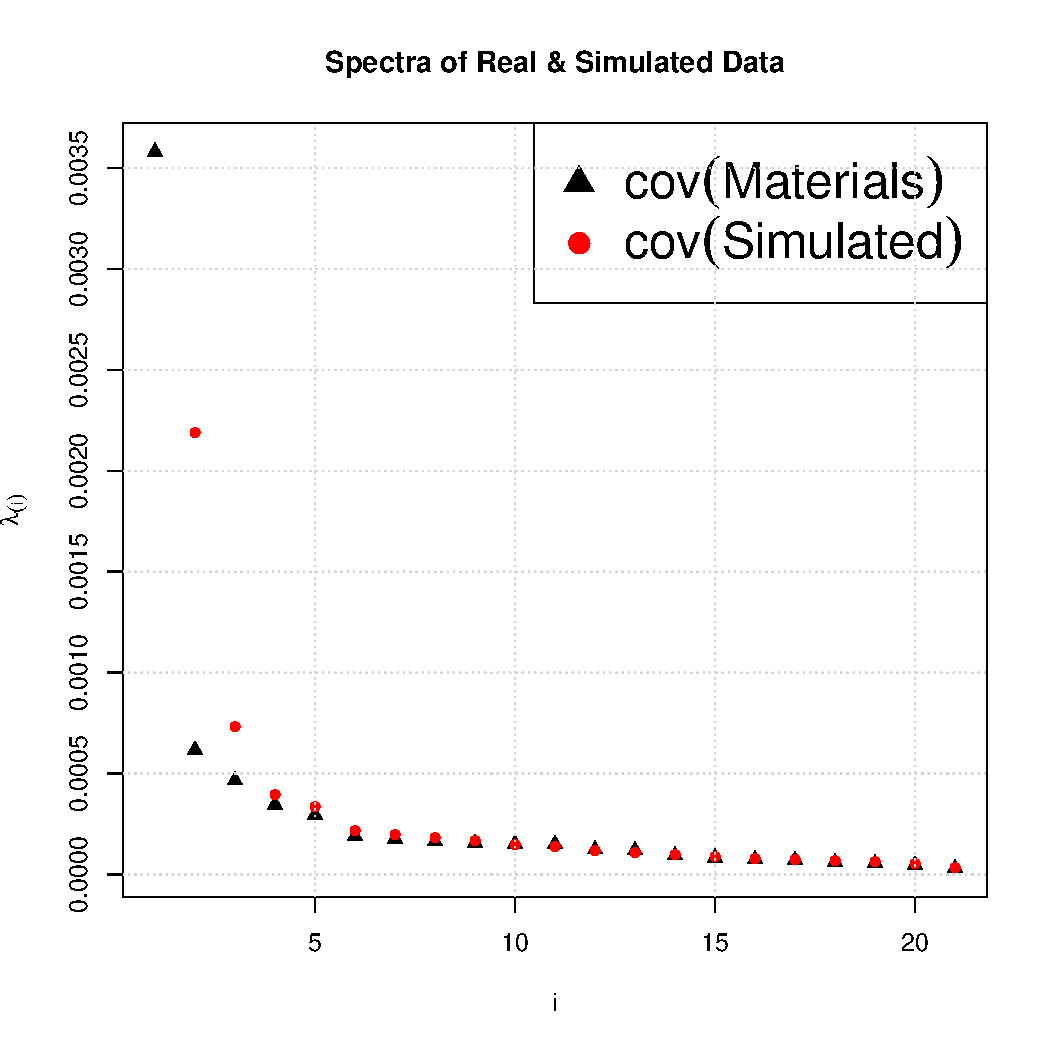
\includegraphics[scale=0.6]{Materials_eigenvalues.pdf}
  \caption{Eigenvalues of Materials: real \& simulated}
  \label{fig:Materials_eigenvalues}
\end{figure}

\begin{figure}[htb!]
  \centering
  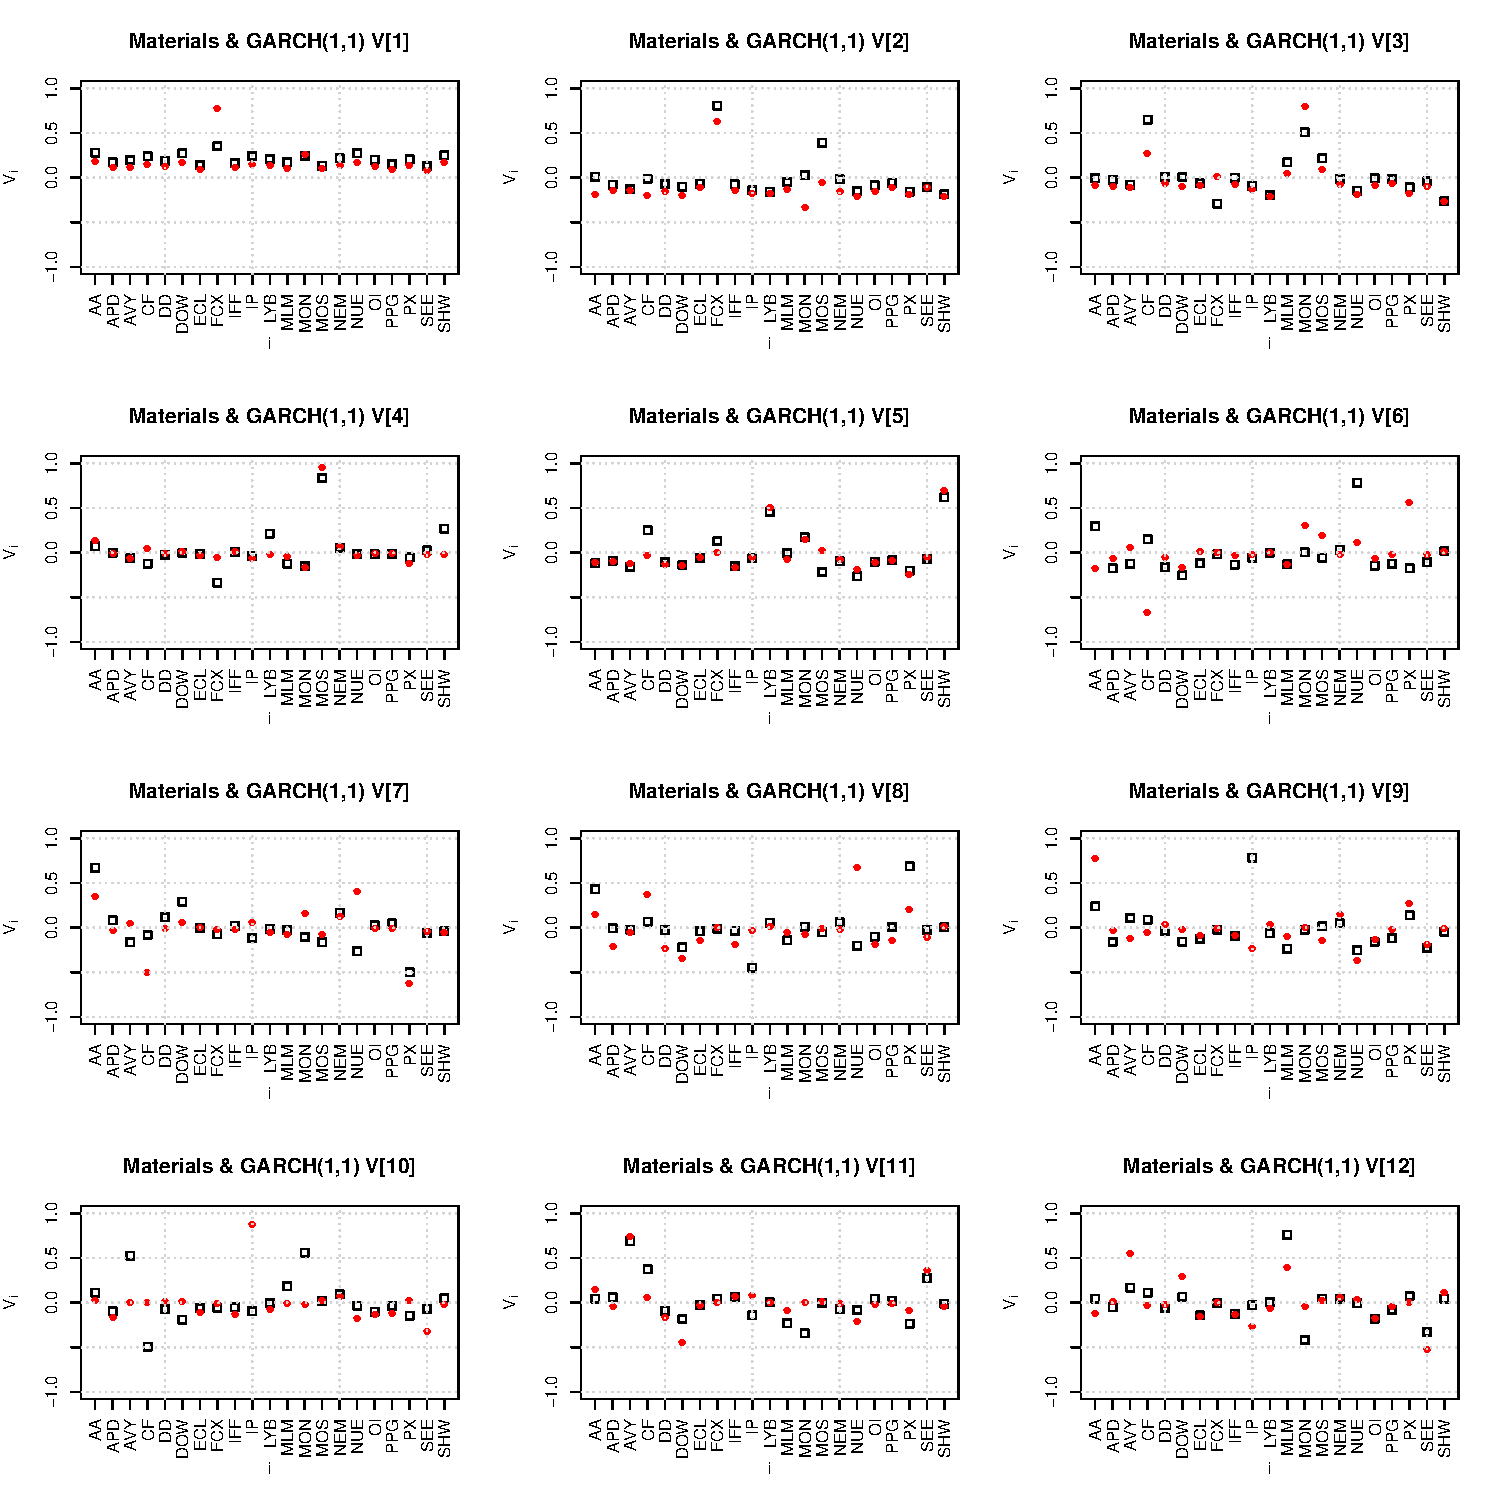
\includegraphics[scale=0.5]{Materials_eigenvectors1.pdf}
  \caption{Eigenvectors of Materials: real \& simulated}
  \label{fig:Materials_eigenvectors1}
\end{figure}

\begin{figure}[htb!]
  \centering
  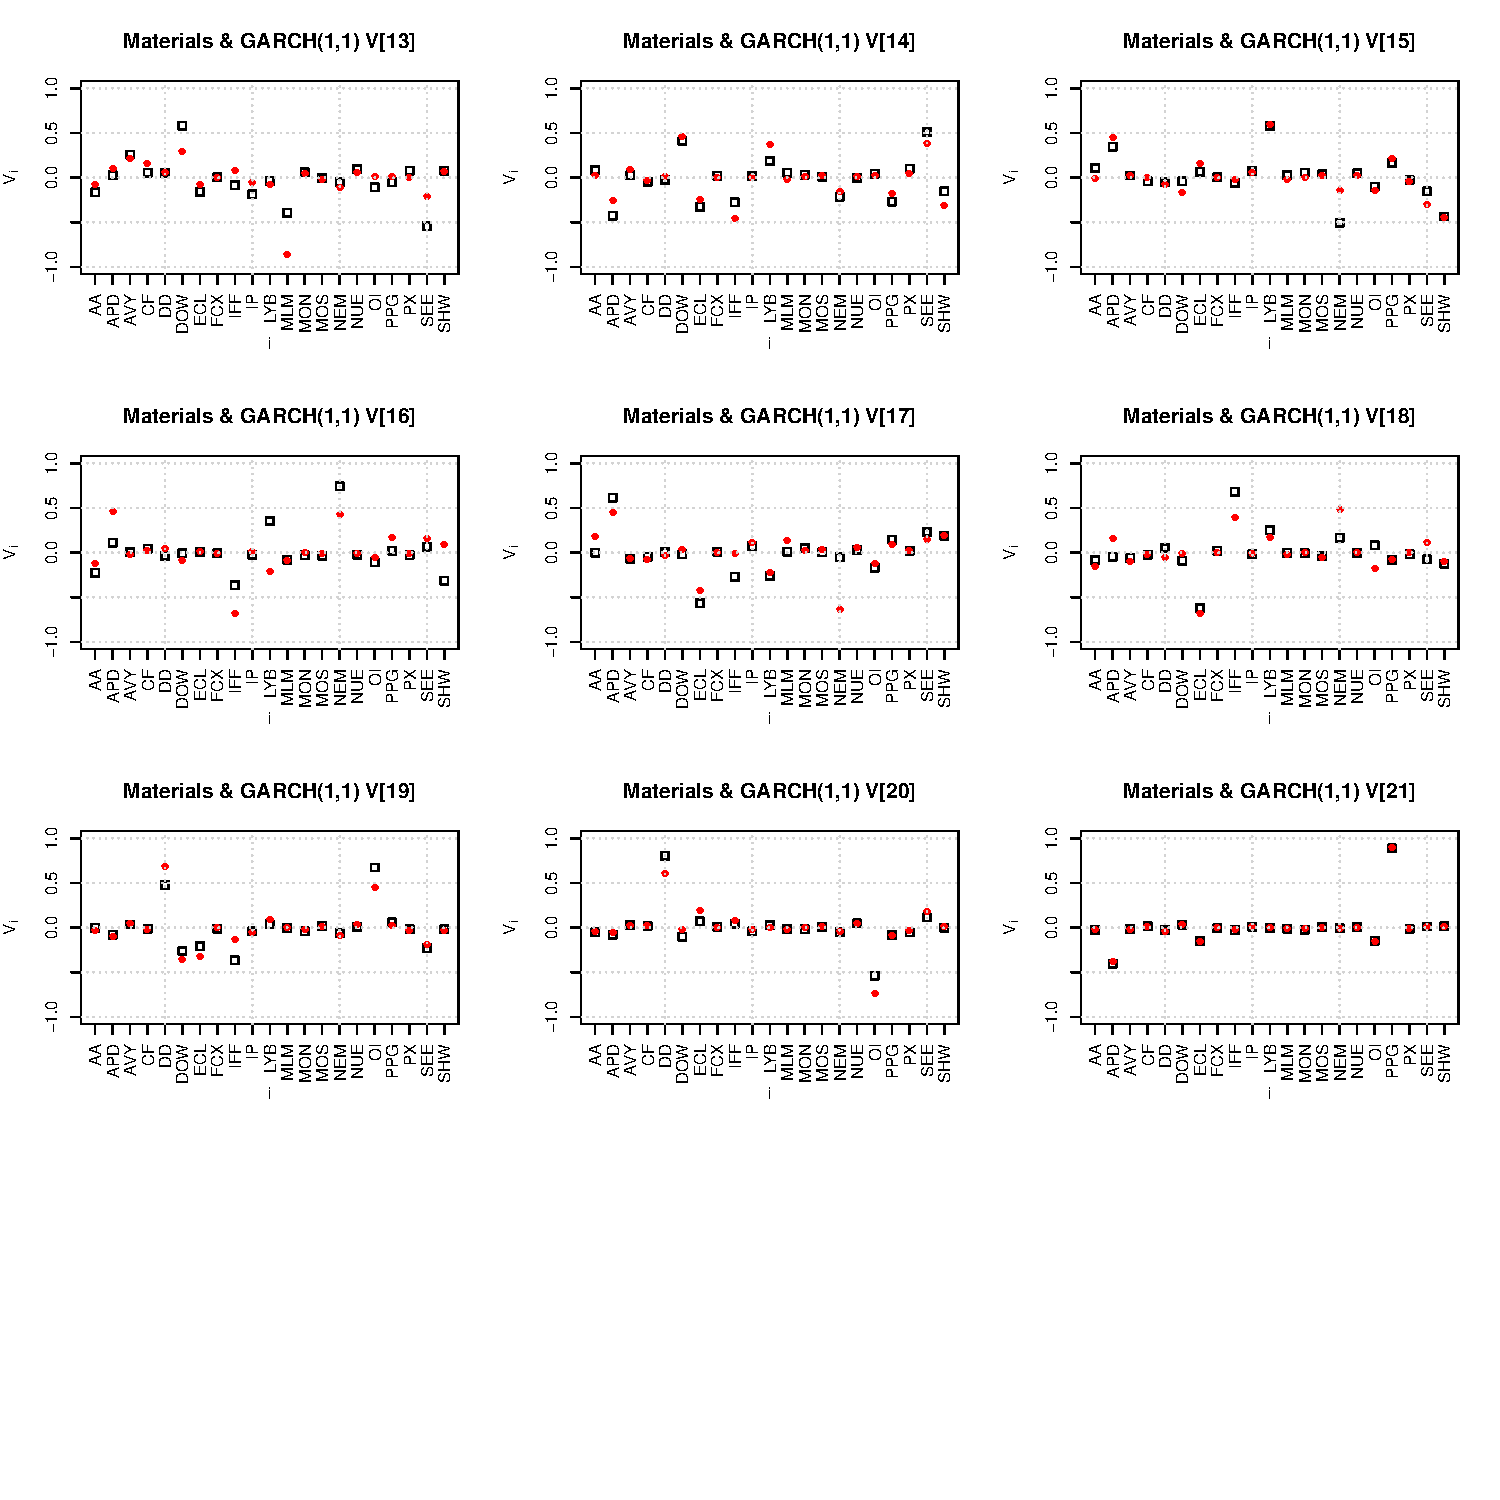
\includegraphics[scale=0.5]{Materials_eigenvectors2.pdf}
  \caption{Eigenvectors of Materials: real \& simulated continued}
  \label{fig:Materials_eigenvectors2}
\end{figure}

\section{Factor Models}
\begin{eqnarray*}
  X_{i,t} &=& \sum_{k=1}^N C_{i,k} Y_{k,t} \\
  Y_{k,t} &=& Z_{k,t} \sigma_{k,t} \\
  \sigma_{k,t}^2 &=& \omega_k + \alpha_k Y_{k, t-1}^2 +
  \beta_{k, t-1} \sigma_{k, t-1}^2
\end{eqnarray*}

Figures \ref{fig:FX_eigenvalues_factor} and
\ref{fig:FX_eigenvectors_factor} show how the spectrum produced by
simulation according to the factor model compares to the spectrum
of real FX data.

\subsection{Orthogonal GARCH}
Kariya (1988) and Alexander and Chibumba (1997) proposed the
orthogonal GARCH model, which treats each sequence as a linear
combination of a number of common, indepdent factors, each of which
is modeled by a variant of GARCH, e.g. standard GARCH,
EGARCH, GJR-GARCH, etc. Figure \ref{fig:FX_eigenvalues_factor} and
\ref{fig:FX_eigenvectors_factor} show the spectrum of real FX data
together with a spectrum of data simulated from the orthogonal GARCH
model. Here the innovations of the GARCH model are sampled from the
$N(0, 1)$ distribution.

GARCH parameters of the factors are estimated from the data, i.e. the
sample covariance matrix of the observed series $X_{i,t}$ are first
computed. The eigenvalues $\lambda_i$ and the eigenvectors $\vec{C_j}$
of the sample covariane matrix are then computed. Let $C_{i,j}$
denote the $i$-th element of the $j$-th eigenvector. Then the $j$-th
factor $Y_{j,t}$ is constructed as
\[
Y_{j,t} = \sum_{i=1} C_{i, j} X_{i, t}
\]
\begin{figure}[htb!]
  \centering
  \includegraphics[scale=0.4]{FX_eigenvalues_factor.pdf}  
  \caption{FX \& simulated GARCH eigenvalues. normal innovations}
  \label{fig:FX_eigenvalues_factor}
\end{figure}

\begin{figure}[htb!]
  \centering
  \includegraphics[scale=0.3]{FX_eigenvectors_factor.pdf}  
  \caption{FX \& simulated GARCH eigenvectors. normal innovations}
  \label{fig:FX_eigenvectors_factor}
\end{figure}

If, however, the innovations are sampled from the Students' t
distribution with degree of freedom estimated from the data, the
simulated spectrum demonstrates a dominance pattern, as shown in
figure \ref{fig:GARCH-t_eigenvalues} and
\ref{fig:GARCH-t_eigenvectors}
\begin{figure}[htb!]
  \centering
  \includegraphics[scale=0.4]{GARCH-t_eigenvalues.pdf}  
  \caption{FX \& simulated GARCH eigenvalues. t-innovations}
  \label{fig:GARCH-t_eigenvalues}
\end{figure}

\begin{figure}[htb!]
  \centering
  \includegraphics[scale=0.3]{GARCH-t_eigenvectors.pdf}  
  \caption{FX \& simulated GARCH eigenvectors. t-innovations}
  \label{fig:GARCH-t_eigenvectors}
\end{figure}


\subsection{Non-linear Factor Model}
A survey of Hill estimated tail indices of 16 currencies are listed in
table \ref{tab:currencies_hill_estimate}. It is visible that Asian
currencies are associated with lower tail indices than are their
counterparts in Europe, North America and Oceania. This observation is
in contradition with classical factor models, by which all the
currencies should have the same tail index that is equal to the lowest
tail index of the factors, since the return series of each currency is
a linear combination of the return series of the factors. The
conclusion follows immediately from Mikosch 2013 \cite{Mikosch2013},
lemma 3.1.
\begin{table}[htb!]
  \begin{tabular}{lr|lr|lr|lr}
    \multicolumn{2}{c|}{Asia} & \multicolumn{2}{|c}{Europe} &
    \multicolumn{2}{|c}{N. America} & \multicolumn{2}{|c}{Oceania}\\
    \hline
    HKD & 1.88 & EUR & 2.09 & CAD & 2.14 & AUD & 2.13 \\
    JPY & 1.92 & NOK & 2.02 & USD & 2.23 & NZD & 2.17 \\
    KRW & 1.98 & CZK & 2.17 & & & &\\
    SGD & 1.98 & DKK & 2.13 & & & & \\
    & &          GBP & 2.21 & & & & \\
    & &          HUF & 2.11 & & & &
  \end{tabular}
  \caption{Hill estimates of currency tail indices by continents}
  \label{tab:currencies_hill_estimate}
\end{table}

Therefore we propose
\begin{eqnarray*}
  X_{i,t} &=& \sum_{k=1}^N C_{i,k} \text{sgn}(Y_{k,t}) |Y_{k,t}|^{\delta_{i,k}}
\end{eqnarray*}
where $0 < \delta_{i,k} \leq 1$ for all $i, k$. In particular, if
currencies $i_1, i_2, ..., i_m$ belong to the same group, e.g. the
group of Asian currencies, $\delta_{i_1, k} = \delta_{i_2, k} = \cdots
\delta_{i_m, k}$.

\section{different tail indices or same tail index but different scales}
The Hill estimator is rather inaccurate in estimating the tail index
of a heavy-tailed series, particularly when the series is scaled
differently. Figure \ref{fig:simulated.indices} shows the Hill
estimates of two groups of simulated series of the form
$X_{i,t} = C_i Y_{i, t} + G_t$, where the series 
$Y_{i}$ and the common factor $G$ are independent and identical
GARCH(1,1) processes. The first, shown in black squares, has $C_i$
ranging from 0.1 to 1.5; the second, shown in red circles, has
$C_i = 1$ for all $i$.
\begin{figure}[htb!]
  \includegraphics[scale=0.5]{simulated_indices.pdf}
  \caption{Tail indices of linearly combined GARCH(1, 1) processes}
  \label{fig:simulated.indices}
\end{figure}


%% Show simulation result of the tail index and scale using the script
%% tail_indices_compare.r
%% Use Hill estimators for both the tail index and the scale
%% Use the optimal number of order statistics as given in Casper's
%% paper.
%% Maybe also show simulation result of the tail index and scale using
%% iid Student's t series.

%% CAUTION: Chen Zhou believes it is hopeless to answer definitely
%% whether two series have the same tail index.



\bibliographystyle{unsrt}
\bibliography{../../thesis/econophysics}
\end{document}
